\documentclass[output=paper]{langscibook}
\IfFileExists{../localcommands.tex}{
  \addbibresource{../localbibliography.bib}
  \usepackage{tabularx,multicol}
\usepackage{url}
\urlstyle{same}
\usepackage{multirow}

\usepackage{stmaryrd}
\usepackage{soul}
\usepackage{enumitem}

\usepackage{siunitx}
\sisetup{group-digits=none}

\usepackage{langsci-optional}
\usepackage{langsci-lgr}
\usepackage{langsci-textipa}
\usepackage{langsci-branding}

\usepackage{tikz-qtree}

\usepackage{pgfplots}
\usepackage{qtree}
\qtreecenterfalse
\usepackage{tree-dvips}
\usepackage{subcaption}

\let\clipbox\undefined
\usepackage{adjustbox}
\usepackage[linguistics, edges]{forest}
\usepackage{langsci-gb4e}

% ORCIDs in langsci-affiliations 
\usepackage{orcidlink}
\SetupAffiliations{orcid placement=before}
\definecolor{orcidlogocol}{cmyk}{0,0,0,1}
\RenewDocumentCommand{\LinkToORCIDinAffiliations}{ +m }
  {%
    \orcidlink{#1}\,%
  }

  \newcommand*{\orcid}[1]{}


\makeatletter
\let\thetitle\@title
\let\theauthor\@author
\makeatother

\newcommand{\togglepaper}[1][0]{
   \bibliography{../localbibliography}
   \papernote{\scriptsize\normalfont
     \theauthor.
     \titleTemp.
     To appear in:
     E. Di Tor \& Herr Rausgeberin (ed.).
     Booktitle in localcommands.tex.
     Berlin: Language Science Press. [preliminary page numbering]
   }
   \pagenumbering{roman}
   \setcounter{chapter}{#1}
   \addtocounter{chapter}{-1}
}

\newbool{bookcompile}
\booltrue{bookcompile}
\newcommand{\bookorchapter}[2]{\ifbool{bookcompile}{#1}{#2}}


\forestset{
  my nice empty nodes/.style={% modified from manual page 52
    for tree={
      calign=fixed edge angles,
      calign angle=50,
    },
    delay={
      where n children=0{
        if content={}{
          content=\strut,
          anchor=north,
        }{
          align=center
        },
      }{
        if content={}{
          shape=coordinate,
          for parent={
            for children={
              anchor=north
            }
          }
        }{}
      }
    },
  },
  my pretty nice empty nodes/.style={
    for tree={
      calign=fixed edge angles,
      calign angle=50,
      parent anchor=south,
      delay={
        where n children=0{
          if content={}{
            content=\strut,
            anchor=north,
          }{
            align=center
          },
        }{
          if content={}{
            inner sep=0pt,
            edge path={\noexpand\path [\forestoption{edge}] (!u.parent anchor) -- (.south)\forestoption{edge label};}
          }{}
        }
      }
    }
  }
}


\newcommand{\sem}[1]{\mbox{$[\![$#1$]\!]$}}
\newcommand{\type}[1]{\ensuremath{\left \langle #1 \right \rangle }}
\newcommand{\lam}{\ensuremath{\lambda}}
\renewcommand{\and}{$\wedge$ }
\newcommand{\bex}{\begin{exe}}
\newcommand{\eex}{\end{exe}}
\newcommand{\bit}{\begin{itemize}}
\newcommand{\eit}{\end{itemize}}
\newcommand{\ben}{\begin{enumerate}}
\newcommand{\een}{\end{enumerate}}

\newcommand{\gcs}[1]{\textcolor{blue}{[gcs: #1]}}
\newcommand{\ash}[1]{\textcolor{orange}{[ash: #1]}}
\newcommand{\ngn}[1]{\textcolor{purple}{[ngn: #1]}}

\newcommand{\firstrefdash}{}


\forestset{
fairly nice empty nodes/.style={
delay={where content={}
{shape=coordinate, for siblings={anchor=north}}{}},
for tree={s sep=4mm}
}
}



  %% hyphenation points for line breaks
%% Normally, automatic hyphenation in LaTeX is very good
%% If a word is mis-hyphenated, add it to this file
%%
%% add information to TeX file before \begin{document} with:
%% %% hyphenation points for line breaks
%% Normally, automatic hyphenation in LaTeX is very good
%% If a word is mis-hyphenated, add it to this file
%%
%% add information to TeX file before \begin{document} with:
%% %% hyphenation points for line breaks
%% Normally, automatic hyphenation in LaTeX is very good
%% If a word is mis-hyphenated, add it to this file
%%
%% add information to TeX file before \begin{document} with:
%% \include{localhyphenation}
\hyphenation{
    par-a-digm
    peri-phras-tic
    mor-pho-pho-nol-o-gy
}

\hyphenation{
    par-a-digm
    peri-phras-tic
    mor-pho-pho-nol-o-gy
}

\hyphenation{
    par-a-digm
    peri-phras-tic
    mor-pho-pho-nol-o-gy
}

  \togglepaper[1]%%chapternumber
}{}

\ChapterDOI{10.5281/zenodo.12090443}
\abstract{Heritage languages are often of interest because of the ways in which they differ from the relevant baseline. Many conceive of these differences as a process of simplification: a loss of inflectional morphology, less lexical richness, etc. Inspired by findings in the literature that decreased complexity in one area of a language may lead to increased complexity in another, we take up the question of whether the changes during the development of heritage languages involve a general simplification, or whether complexity trades off in heritage languages as it does in other languages: as speakers rely less on word-internal structure, word order matters more, and vice versa. We apply information-theoretic measures of complexity in the domain of word structure (i.e., morphology) and word order (i.e., syntax) to six languages from the Heritage Language Documentation Corpus \citep{nagy2011}, which includes multiple generations of heritage languages and homeland comparators. Our results show partial support for complexity trade-offs in heritage languages, such that as the generations progress, word-structure complexity decreases while word-order complexity increases.
\keywords{heritage language; complexity; word structure; word order; trade-off}
}
\title{A multi-generational analysis of heritage language complexity}
\author{Ashvini Varatharaj\affiliation{University of California, Santa Barbara} and Gregory Scontras\affiliation{University of California, Irvine} and Naomi Nagy\affiliation{University of Toronto}}


\begin{document}
\maketitle
\section{Introduction}
\begin{sloppypar}
Languages can be complex in various ways. Existing attempts at objectively quantifying grammatical complexity have primarily focused on morpho-syntactic components, either word-internal structure or the complexity introduced by word order restrictions.
Some of these studies calculate complexity on the basis of hand-coded grammatical features \citep[e.g.,][]{shosted2006correlating,lupyandale2010}, while others use computational or  information-theoretic metrics 
to calculate the complexity of a grammar based on the behavior that grammar generates (i.e., naturalistic productions from corpora; e.g.,  \citealp{juola1998measuring,koplenig2017statistical}). We examine the second type of complexity in this paper.
\end{sloppypar}

Importantly, complexity is not a static quantity; the complexity of different grammatical components may shift over time. Complexity also differs across levels of a language. Indeed, a prominent (though problematic) view in language science holds that all languages are equally complex, such that language change involves the redistribution of complexity from one aspect of a language to another. According to this law of conservation of complexity, as it were, complexity can neither be created nor destroyed. While we hesitate to adopt a strong version of this stance (for discussion, see \citealp{sampson2009language}), we do believe the perspective offers lessons that may help guide inquiry: while total complexity may not be a static quantity, there are likely to be interactions between grammatical components such that increases of complexity in one domain may lead to (or coincide with) decreases in others. Existing investigations have approached these interactions primarily through the lens of idealized monolingualism; the current work investigates complexity in the area of heritage languages.

Heritage speakers are bilinguals who learn their first language (the heritage language) at home. They may then shift to speak the dominant societal language, typically at the onset of schooling \citep{rothman2009,scontrasetal2015frontiers,PolinskyScontras2020}. 
Children usually acquire a heritage language from their parents, who are often recent immigrants. 
Impressionistically, heritage languages are commonly described in terms of decreased complexity: fewer morphological distinctions, a more limited syntactic repertoire, etc.~(see \citealp{polinsky2018book} for discussion). 
Here, we call into question the notion that the process of becoming a heritage language involves only simplification, looking at how complexity changes as a language develops from homeland speakers through successive generations of heritage speakers. 
Our aim is to understand how (or if) changing complexity in one area of a language (say, word-structure or morphological complexity) interacts with complexity in other areas of the language (say, word-order or syntactic complexity). To accomplish this aim, we use multi-generational data collected as part of the Heritage Language Variation and Change Project (i.e., the largest attempt at documenting multi-generational heritage language productions; \citealp{nagy2009heritage}), applying off-the-shelf information-theoretic metrics of complexity to transcribed naturalistic speech from six heritage languages: Cantonese, Faetar, Italian, Korean, Russian and Ukrainian.

In Section \ref{background}, we provide background on information-theoretic measures of complexity. In Section \ref{method}, we present the complexity metrics we use in more detail, together with an overview of the data to be analyzed; we then present our results and follow-up analyses in Section \ref{results}.  
We conclude in Section \ref{discussion} with a discussion of our findings in light of the literature on heritage language and grammatical complexity, noting that our preliminary findings support a trade-off between morphological and syntactic complexity that develops from one generation of heritage speakers to the next.


\section{Background}
\label{background}

Opinions about language complexity abound. An English speaker trying to track gender on the nouns of Spanish might suspect that the Spanish nominal system features more complexity than English's; a Spanish speaker attempting to internalize the Russian declension system would likely conclude that Spanish's two genders hardly compete with Russian's six cases. But L1 speakers all wind up acquiring the relevant systems, so does any of these languages count as more complex than the others? Despite the abundance of anecdotal intuitions, the trick lies in operationalizing complexity so that it may be subjected to objective -- or at least systematic, reproducible -- measurement. The first step often involves relativizing complexity to specific aspects of a language or components of its grammar. In what follows, we review several attempts at such an operationalization of complexity.

Our focus is on grammatical complexity, or the complexity of the language-specific knowledge a speaker possesses when they know a language. Other types of complexity focus on the use of the linguistic system; while there are many interesting questions to pose about user-based complexity in heritage languages (for discussion, see \citealp{lalekoscontras2021}), we limit our focus to the complexity of the linguistic system itself. Now, assessments of grammatical complexity are necessarily indirect, owing to the fact that comprehensive descriptions of linguistic knowledge -- in other words, fully-specified grammars -- have yet to be identified. As is common in (socio)linguistics, we consider performance in communicative tasks as an accessible proxy of this competence. The indirectness enters, then, in the inference of a grammar's content on the basis of the observable linguistic behavior the grammar generates. We may use the observable behavior to construct partial grammars, and then evaluate their complexity via various forms of counting (e.g., \citealp{nichols1992,bakker1998,lupyandale2010}). Or we may skip the partial grammars altogether and directly evaluate the complexity of observed language behavior, with the assumption that the more complex the behavior is, the more complex the grammar that generated it must be. We will focus on this latter approach, applying complexity metrics directly to naturalistic corpora (i.e., the behavior generated by some grammar(s)) in an effort to assess grammatical complexity.

Corpus-based approaches offer a fast and reproducible method to calculate complexity, with the advantage that there is no need for hand-coding grammatical features of the language under investigation. In other words, corpus-based approaches lessen the need for (and potential bias introduced by) intuitions of the investigator. These methods were initially focused on morphological complexity; they are founded on the idea that morphological complexity depends on the morphological component of a language's generative grammar, which determines the language's inflectional and derivational processes. A productive system will produce different but related word forms (e.g., \emph{walk} and \emph{walked}); as the number of morphological relationships among word forms -- and the irregularity of those relationships -- increases, so too does the complexity of that system. Information-theoretic metrics can provide us with an understanding of this morphological richness \citep{gutierrez2020productivity}.

Here we review two studies that have inspired our current work. In the first, \citet{juola1998measuring} pioneers a metric for estimating morphological complexity. \citeauthor{juola1998measuring} identifies complexity with compressibility -- or, more precisely, with the lack of compressibility. A more complex string of text will carry more information; it will also be less compressible, because it will require a more complex system to encode and reconstruct (or generate) the original string. This notion of complexity relates to the information-theoretic notion of Kolmogorov complexity \citep{kolmogorov1968,livitanyi2008}, where the complexity of a grammar is a function of the length of the minimal description (i.e., specification) of the grammar. \citeauthor{juola1998measuring} recognized that comparison between the amount of morphological information in an original text and in a altered version of the text (without morphological structure) can constitute a measure of the informativeness of the text, and thereby the amount of information encoded morphologically. By estimating the amount of information conveyed by morphology (i.e., word structure), \citeauthor{juola1998measuring} arrives at a method for estimating complexity of the morphological tier of the grammar.

In more detail, \citeauthor{juola1998measuring} artificially inflated the information content of the morphological tier by replacing each word type in a corpus with a unique number. So, \emph{walk} may be replaced by the number 139 and \emph{walked} by 4597. While a compression algorithm can seize on the transparent morphological relationship between \emph{walk} and \emph{walked}, that relationship is destroyed in the case of 139 and 4597; the resulting text with words replaced by numbers is thus less compressible, which means it is more complex. Inflating morphological complexity becomes more difficult as the morphology becomes less regular; \emph{see} and \emph{saw} have little redundancy for a compression algorithm to seize on, and so replacing the words with random numbers does little to increase complexity. 

A ratio of compressed text size between the original text and the mor\-phol\-og\-i\-cal-struc\-ture-de\-stroyed text gets used as an approximate measure of morphological complexity. We describe \citeauthor{juola1998measuring}'s methodology in more detail in the following section; for now, the key to this approach is the fact that, by inflating the information content of the morphological tier, languages with regular, simple morphology will have their information content greatly increased relative to the information in the unaltered text, thus providing a numerical measure to compare morphological complexity across different languages. 

\citeauthor{juola1998measuring} applied his metric to Bible translations in six languages: Dutch, English, Finnish, French, Maori, and Russian. Because they communicate the same message, the Bible translations control for overall message complexity; any differences in compressibility across languages are assumed to result from the complexity of message encoding, which an individual language's grammar determines. \citeauthor{juola1998measuring} found that the six languages are ordered as follows with respect to morphological complexity: 

\ea {Maori} <  {English} <  {Dutch} <  {French} <  {Russian} <  {Finnish}\z

Crucially, the results of \citeauthor{juola1998measuring}'s compression-based complexity metric align with those of \citet{nichols1992}, who hand-calculated morphological complexity by counting the number of points at which typical sentences may be inflected in a given language.

In the second study that directly informs our own investigation, \citet{koplenig2017statistical} implement an entropy-based variant of \citeauthor{juola1998measuring}'s metric to estimate both morphological and syntactic complexity, looking for trade-offs between the two quantities across languages in the Parallel Bible Corpus \citep{mayer2014creating}. The authors assess intra-lexical and inter-lexical regularities and show that there is a negative correlation between the two: as word-order complexity increases across languages, word-structure complexity decreases, and vice-versa (see also \citealp{juola2008assessing}). A particularly interesting result is the observation regarding the diachronic complexity trade-offs within a single language: English. \citeauthor{koplenig2017statistical}~use their metrics to show that as English changes from Old English to Middle English, Modern English, and then to English-based Creole, information present in word structure decreases, and word-order information increases. In other words, as the morphology simplifies in the historical development of English such that less information gets communicated via morphology, the information that would have been communicated via morphology gets carried instead by word order. In our work, we study similar relationships between word-structure and word-order complexity in the development of heritage languages, from speakers in the homeland through subsequent generations of heritage speakers.



\section{Methodology} \label{method}
Here we discuss our dataset and the methods we used to assess grammatical complexity.

\subsection{Data}

The dataset used is obtained from the Heritage Language Variation and Change Project (HLVC; \citealp{nagy2009heritage}), which examines usage and change in  heritage -- that is, non-official -- languages spoken in the Greater Toronto Area. The Heritage Language Documentation Corpus (HerLD) documents cross-generational variation in ten heritage languages via digital recordings of spontaneous conversational speech and time-aligned orthographic transcriptions of these conversations. The corpus contains transcriptions of sociolinguistic interviews of about one hour in length and a picture-description task, 10–15 minutes, describing pictures from a children's book called \emph{First 100 Words} \citep{amery1987first}, as well as coded responses to an ethnic orientation questionnaire. For each language, adult heritage language speakers are recorded to represent four generational groups, defined as follows:\largerpage

\begin{description}
\item[Homeland:] 
\begin{itemize}
\item[]
\item born in the homeland and remained there
\end{itemize}
\item[1st generation (Gen 1):]
\begin{itemize}
 \item[]
 \item born in the homeland 
 \item moved to the Greater Toronto Area after age 18
 \item in Toronto at least 20 years
 \end{itemize}
\item[2nd generation (Gen 2):]
\begin{itemize}
  \item []
  \item born in the Greater Toronto Area (or came from homeland before age 6)
  \item parents qualify as 1st generation
  \end{itemize}
\item[3rd generation (Gen 3):]
\begin{itemize}
 \item []
 \item born in the Greater Toronto Area
 \item parents qualify as 2nd generation
 \end{itemize}
\end{description}

One additional inclusion criterion is that participants self-identify as fluent enough to participate in a one-hour conversation in their heritage language. Data were collected by heritage speakers, recruiting through their personal networks. No fluency or proficiency tests were administered, and participants were selected to represent a diverse array of backgrounds. They vary in terms of education, language attitudes, frequency of language use, etc. More information about the speakers and their selection can be found in \citet{nagy2011, nagy2015sociolinguistic,nagy24}. Details about data collection are available at \url{https://ngn.artsci.utoronto.ca/HLVC/2_2_linguists.php}. For Ukrainian, it has been possible to collect small samples of Gen~4 and Gen~5 speakers. For the Asian languages, there is limited availability of third-generation speakers due to strict immigration restrictions until the 1960's. 
\tabref{table:basic_stats} shows the distribution of languages and speakers selected for our analyses. 

\begin{table}
\begin{tabular}{lrrrrrrr}
\lsptoprule
  & \multicolumn{7}{c}{{Generation}} \\\cmidrule(lr){2-7}
{Language}  & {H} & {1} & {2} & {3} & {4} & {5} & {Total} \\\midrule
{Cantonese} & -   & 2          & 2          & 2          & -          & -          & 6              \\
{Faetar}    & -   & 9          & 9          & -          & -          & -          & 18             \\
{Italian}   & -   & 5          & 14         & 7          & -          & -          & 26             \\
{Korean}    & 7   & 3          & 9          & 1          & -          & -          & 20             \\
{Russian}   & -   & 11         & 15         & 3          & -          & -          & 29             \\
{Ukrainian} & 18  & 3          & 7          & 7          & 3          & 1          & 39             \\
\lspbottomrule
\end{tabular}
\caption{Number of speakers for each language across generations. H: Homeland generation.}
\label{table:basic_stats}
\end{table}


\subsection{Metrics}

Our complexity metric comes from the work of \citet{juola1998measuring}, where the in\-for\-ma\-tion-the\-o\-ret\-ic idea of using a compression-based metric for measuring language complexity was proposed. To understand the metric used in this work, one needs to first understand how to quantify information. According to information theory, “information” is the amount of surprisal or unexpectedness present in a text sample -- in other words, the extent to which the text is not easily predictable. (If the contents of a text are predictable, then the information it would have conveyed is already in hand, so the text contributes little new information.) The common model to measure information is in the form of transmitting messages (usually treated as stochastic, i.e., randomly determined, or having a random probability distribution or pattern that may be analyzed statistically but may not be predicted precisely) from a source to a listener through some channel. The transmitter encodes the message (in our case, in the form of some text); the listener decodes the message. If the probability distribution for the source producing these messages is known, then we can find an encoding method that transmits the messages with maximum efficiency.\footnote{By ``maximum efficiency'' we mean that the system is able to transmit the entire message to the receiver without any loss of information, since the source probabilities are known and lost information can be easily recovered.} This encoding efficiency is known as Shannon’s entropy, calculated by the equation 
$H = -\sum_{i=1}^{n}p_{i} \log ( p_{i} )$
where $p_i$ is the probability of the $i$th message being transmitted (given that there are \textit{n} messages to be transmitted). In real-world scenarios, the exact probabilities are not known but only approximated using different methods \citep{ziv1977universal, ziv1978compression}, which gives an indirect estimation of entropy. Higher-entropy distributions feature greater uncertainty; samples from these distributions are less predictable, which means that encountering one of those samples is more informative.

Next, we must understand what compression means in this context. The process of compression involves removing repeated (or inconsequential) bits of information to make files smaller, typically by reducing the number of bits (1's and 0's) used to store the information (information in this context is represented as 1’s and 0’s). The main idea of compression within Information Theory is to reduce a communication channel to its maximum efficiency (for example, modern file compression programs use some version of entropy reduction). 

Kolmogorov offers another complexity metric that measures a different aspect of informativeness. Kolmogorov complexity measures the information present in a given string of text 
in terms of the size of the algorithm required to describe that string or regenerate it. The size of the algorithm can be seen as the amount of effort required to transmit the message from source to receiver as assumed in information theory. Intuitively, Shannon’s entropy can be seen as the upper limit of Kolmogorov complexity: a decompression program and a compressed file can be used to (re)generate the original message/string. Thus we can say that a more complex string (in the Kolmogorov sense) will be less compressible and therefore require a larger program and compressed text system to reconstruct. In this way, the compressibility of a text gives us a way to estimate its complexity and the complexity of the grammar that generated it. 

For our work, we utilize the gzip compression algorithm. 
While the algorithm has multiple steps, the most important one for our purposes reduces redundancy. 
This step involves going through the text and, for each sequence of characters, looking back through the text to see if the same sequence of characters has occurred before. If it has, then the algorithm replaces the current occurrence with a pointer in the current location back to the previous occurrence. In other words, the current occurrence gets deleted and replaced by a pointer, and therefore the file size shrinks. 

We calculate \citeauthor{juola1998measuring}'s word-structure complexity metric for our heritage data by first replacing each unique word type in the corpus with a random number (using the Keras Tokenizer; \citealp{chollet2015keras}) to destroy any morphological relationship at the word level, thus trying to increase complexity/decrease compressibility. We refer to this version of the text as the \textit{cooked} version of the text (we borrow this terminology from \citealp{juola1998measuring}; see \tabref{table:example_text} for an example). As mentioned previously, the words \emph{walk} and \emph{walked} would now be replaced with two unrelated random numbers. While the fact that two words are related and have common characters could be used in the raw text's compression, the relationship no longer exists once we replace the words with numbers, thus destroying the morphological relationship between such related words. For each speaker's text (i.e., the transcription of their descriptions of the \emph{First 100 Words} picture book), the original raw text and the cooked text with random numbers are then separately compressed using the gzip compression algorithm. The ratio of these two file sizes is calculated for each speaker, which serves as our metric for word-structure complexity. We refer to this ratio as $R/C$, where R is the size of the compressed raw text, and C is the size of the compressed \textit{cooked} text. 

For an intuitive understanding of the $R/C$ metric of word-structure complexity, consider how the quantity behaves. The compressibility of a cooked file C represents an attempt to inflate the information contained within the morphological tier by destroying relationships across words (e.g., walk~::~walked vs. 139~::~4597). It is easier to artificially inflate morphological information (i.e., increase C) in a language where the morphology does not already contribute substantial information; thus, the ratio of the compressed raw text R to the compressed cooked text C will be smaller (i.e., $R/C$ will decrease). In a language with a rich, informative morphological system, it will not be as easy to inflate morphological information in this way, so C will be smaller relative to R, and thus 
$R/C$ increases. In practice, rich morphological systems with large amounts of irregularity -- in other words, systems that necessitate a longer description -- will yield higher $R/C$ values.

While \citet{juola1998measuring} presents a way to measure morphological complexity in terms of the information content of a language's word structure, this method can easily be extended to analyze word-order complexity; we simply need a method to artificially inflate the information contributed by word order. Just as replacing word types by integers destroys morphological regularities and thereby inflates word-structure complexity, randomly shuffling the order of words destroys word-order regularities and thus inflates word-order complexity (see \tabref{table:example_text} for an example; cf.~\citealp{koplenig2017statistical}). To estimate word-order complexity, we randomly shuffle the words in each speaker's data (i.e., raw text) and then compress the resulting file and calculate the ratio between the raw data and the cooked data with shuffled word order, referring to this value as $R/C\textsubscript{shuffled}$.  
The $R/C\textsubscript{shuffled}$ calculation compares raw to shuffled text; the number-encoded cooked version is not involved.

\begin{table}
\begin{tabularx}{\textwidth}{Ql}
\lsptoprule
{Raw text}       & they walked to the station\\
\tablevspace
Number-encoded cooked text\newline  (increasing morphological complexity) & 13   4597   4   210    190 \\
\tablevspace
 Shuffled cooked text \newline (increasing word-order complexity)      & the station they to walked  \\
\lspbottomrule
\end{tabularx}
\caption{Examples of raw and cooked texts}
\label{table:example_text}
\end{table}

The intuitive understanding of $R/C\textsubscript{shuffled}$ mirrors that of $R/C$: it is easier to artificially inflate the word-order information (i.e., increase C\textsubscript{shuffled}) in a language where word order does not already contribute substantial information. Thus, in a language with low word-order complexity, C\textsubscript{shuffled} will be larger and so $R/C\textsubscript{shuffled}$ will be smaller. In a language with high word-order information, it will be harder to increase the already-high information, and so $R/C\textsubscript{shuffled}$ will be larger. In practice, $R/C\textsubscript{shuffled}$ will increase as a language's word order becomes more rigid, since more space will be required to describe the constraints on order (e.g., \citealp{ehretszmrecsanyi2019}).

We use the correlation between  $R/C\textsubscript{shuffled}$ and $R/C$, as well as the ratio between the two metrics across generations, to make inferences about the relationship between word-order and word-structure complexity across heritage language generations. To assess the amount of variation in our data, we bootstrap confidence intervals by re-sampling the data with replacement \citep{singh2008bootstrap}. For each language, we sample (i.e., randomly select) speaker data (with replacement) of size $n$ (where $n$ is the total number of speakers for that language) and calculate the metrics. We repeat this process for a hundred iterations; where 95\% of the results fall serves as our (bootstrapped) 95\% confidence interval.


\section{Analysis and results} \label{results}

Given the sensitivity of information-theoretic measures of complexity to the amount of data under analysis \citep[e.g.,][]{ehretszmrecsanyi2019}, we begin by presenting the results for Ukrainian, the language for which we have the most data and thus the best chance of finding reliable results (cf.~\tabref{table:basic_stats}). We then expand our analysis to the other languages in our dataset, and in the process we introduce additional analyses to aid in characterizing the pattern of results.

In order to compare more similar content across the heritage languages, we use the speakers' data from the picture-description task for this part of the analysis. Comparable corpora are a valuable resource for many Natural Language Processing tasks and linguistics studies; parallel corpora allow researchers to compare the complexity of message encoding independent from the complexity of the message itself. While not perfectly parallel, the picture-description task data come closer than the sociolinguistic-interview task data to a parallel corpus, given that all speakers were describing the same images. 


\subsection{Ukrainian}

The results of our two complexity metrics are plotted in \figref{ukr_rc}. We see that morphological complexity ($R/C$) is higher in homeland speakers than in heritage speakers. Among the heritage speaker groups, we further see a trade-off between morphological complexity and word-order complexity: as the heritage generation increases, $R/C$ decreases while $R/C\textsubscript{shuffled}$ increases; the two quantities are negatively correlated, and the Spearman correlation reaches significance ($\rho = -0.83$, $p< 0.001$). The value of word-order complexity for the homeland speakers is intermediate between the values of generations 2 and 3. 

\begin{figure}
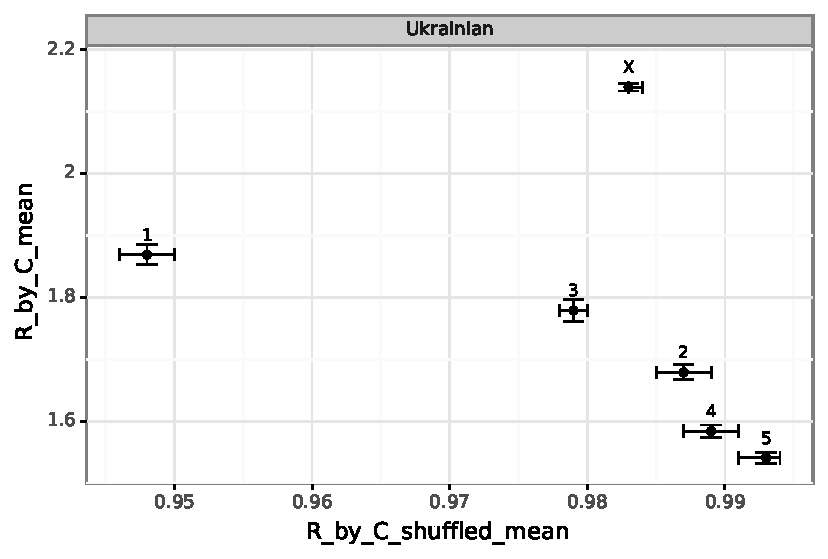
\includegraphics[width=\linewidth]{figures/UKR_ggplot_FW.pdf}
\caption{Ukrainian Language complexity metrics: $R/C$ (i.e., word-structure complexity) vs.~$R/C\textsubscript{shuffled}$ (i.e., word-order complexity). Error bars represent bootstrapped 95\% confidence intervals}
\label{ukr_rc}
\end{figure}

These results suggest that heritage speakers rely less on morphological information to communicate their messages, compared to homeland speakers. And the reliance on morphological information continues to decrease across the generations of heritage speakers. As the information conveyed by word structure decreases, we observe an increase in word-order information among the heritage speakers: the information that would have been communicated by word-internal structure presumably gets shifted to information conveyed by word order. This interpretation is confirmed in \figref{ukr_complexity}, where we plot the ratio between word-structure and word-order complexity across generations. The {complexity ratio} should not be confused with the {complexity metrics} ($R/C$  and $R/C\textsubscript{shuffled}$); the complexity ratio is the ratio of the complexity metrics ($R/C$ $\div$   $R/C\textsubscript{shuffled}$).  As \figref{ukr_complexity} shows, the complexity ratio shifts in favor of word-order complexity as the generations progress away from the homeland ($\rho = -0.94$, $p< 0.001$). 

\begin{figure}
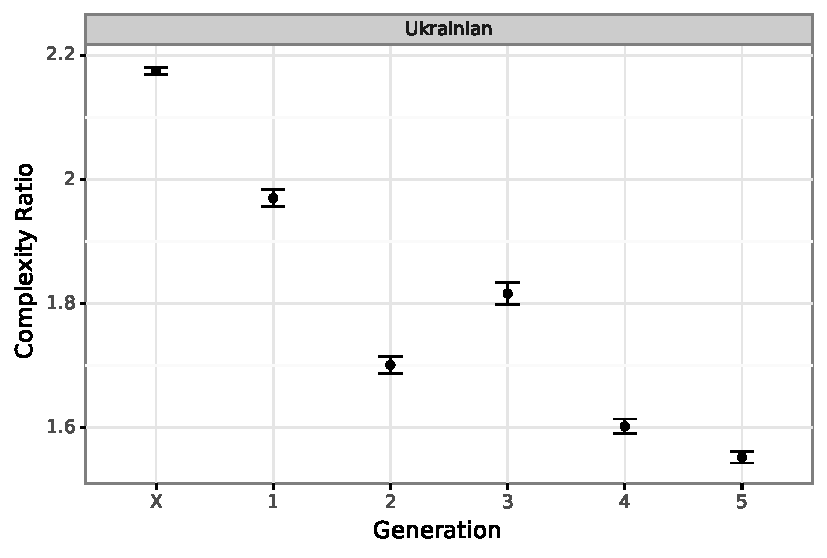
\includegraphics[width=\linewidth]{figures/UKR_ggplot_FW_complexity.pdf}
\caption{Ukrainian language complexity ratio ($R/C$ $\div$   $R/C$\textsubscript{shuffled}) across the generations}
\label{ukr_complexity}
\end{figure}

Despite the clear pattern of complexity shift across the generations, the relative order of generations 2 and 3 defies the general trend away from word-structure complexity. While the difference between these two generations is small, it is worth seeking an explanation, as we find traces of this trend in several languages (see Section \ref{more-languages}). Although the precise source of this pattern remains unclear, a contributing factor could be the change in living conditions in the relevant generations. By the third generation, many families are well-established and able to focus on maintenance of the heritage language alongside English, while the second generation may have felt more pressure to focus resources on English. Also, in some immigrant communities in Toronto, grandchildren often live with (and thus use their heritage language more with) their grandparents while attending university, suggesting another motivation for similarity between first- and third-generation speech.    


\subsection{More languages} \label{more-languages}

For the other languages in our analysis, we have less data to analyze (cf.~\tabref{table:basic_stats}), and so we consider the following results preliminary. Still, some patterns already present themselves. 

\figref{fig:other-languages-r/c} plots word-structure complexity ($R/C$) against word-order complexity ($R/C\textsubscript{shuffled}$) for the remaining languages: Cantonese, Faetar, Italian, Korean and Russian (as well as Ukrainian). No language clearly replicates the trend found in Ukrainian. 
\tabref{fig:corr} reports the statistical correlations, repeating the correlation given above for Ukrainian. We see that Ukrainian, Russian, and Faetar have a negative correlation between $R/C$  vs.~$R/C\textsubscript{shuffled}$, indicating that as word structure increases, information present in word order decreases; these trends are consistent with the findings from \citet{koplenig2017statistical}. However, only in Ukrainian is the correlation significant -- perhaps owing to the smaller datasets for Russian and Faetar.  On the other hand, Italian, Korean, and Cantonese have positive correlations, suggesting that as word-structure information increases (or decreases), word-order information also increases (or decreases) -- precisely the opposite pattern one would expect on the basis of \citeauthor{koplenig2017statistical}'s findings. However, none of these trends reach significance.

\begin{figure}
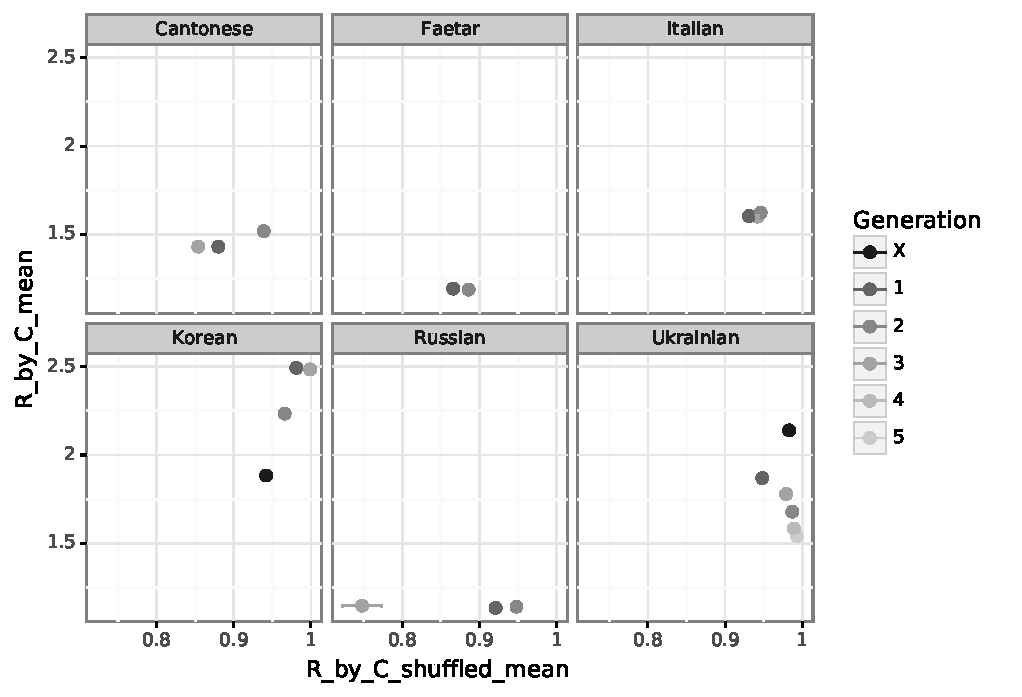
\includegraphics[width=\linewidth]{figures/ggplot_FW_all.pdf}
\caption{%
        $R/C$  vs.~$R/C\textsubscript{shuffled}$ for all languages}%
\label{fig:other-languages-r/c}
\end{figure}

\begin{table}
\begin{tabular}{l S[table-format=-1.2{**}] S[table-format=-1.2{***}]}
\lsptoprule
& {$R/C$ vs.~$R/C\textsubscript{shuffled}$} & {Generation vs.  Ratio} \\
\midrule
Cantonese  & 0.50      & 0.50  \\
Faetar     & -1.00     & -1.00 \\
Italian    & 0.50      & -1.00{***}\\
Korean     & 0.80      & 0.40 \\
Russian    & -0.50     & 0.50  \\
Ukrainian  & -0.83{**} & -0.94{***}\\
\lspbottomrule
\end{tabular}
\caption{Spearman correlation between the complexity metrics ($R/C$ and $R/C\textsubscript{shuffled}$), and between generation and complexity ratio. *** indicates $p < 0.001$,  ** indicates $p < 0.01$, * indicates $p< 0.05$.}
  \label{fig:corr}
\end{table}

To get a better sense of the changing trend across generations, in \figref{fig:other-languages-ratio} we plot the ratio between the two complexity measures across the generations within each language; \tabref{fig:corr} provides the correlations between the generations and the complexity ratio for each language. In addition to Ukrainian, the trend in Italian reaches significance; in both languages we find negative correlations such that, as the generations progress from homeland to later generations, the complexity ratio decreases. In other words, in Ukrainian and Italian, but not the other four languages, we find evidence supporting complexity trade-offs in favor of word-order complexity across generations. While the Italian trend is difficult to read off of \figref{fig:other-languages-ratio} given the y-axis scale, the statistics in \tabref{fig:corr} support the reliability of this relationship.

\begin{figure}[t]
\centerline{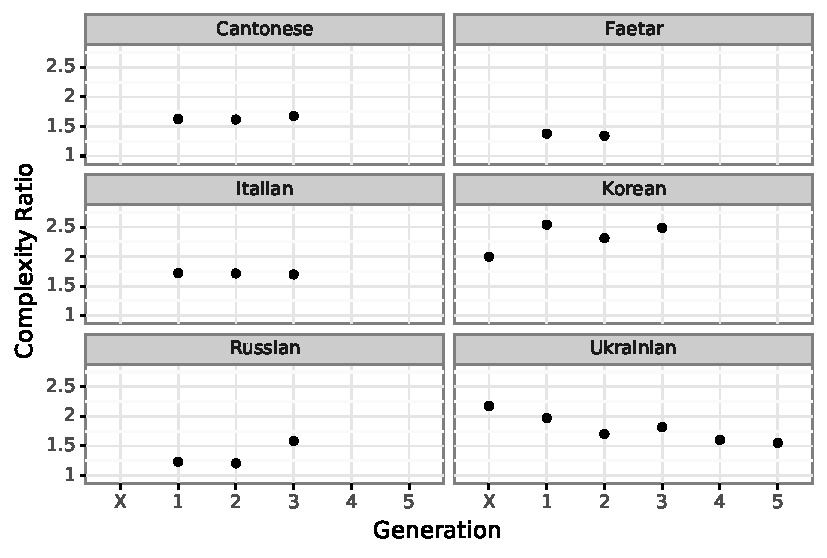
\includegraphics[width=\linewidth]{figures/All_ggplot_complexity.pdf}}
\caption{Complexity ratio across generations for all languages: $R/C$ $\div$   $R/C\textsubscript{shuffled}$}
\label{fig:other-languages-ratio}
\end{figure}

The ratio analysis also sheds some light on the non-significant positive correlations observed between word-order and word-structure complexity. Although we find trends such that word-order and word-structure complexity increase or decrease with each other (as seen in \figref{fig:corr}), these increases and decreases do not track the generations of heritage speakers (as seen in \figref{fig:other-languages-ratio}).


\subsection{Followup analysis: Parallel Bible Corpus}

Having found clear evidence of a complexity trade-off in Ukrainian and partial evidence in Italian, we decided to explore what might set Ukrainian apart -- and in the process also verify the behavior of our metrics. The most obvious explanation for the behavior of Ukrainian vs.~the other languages in our study is that we have the most data for Ukrainian, and so it is the only language for which we can get a clear picture of the changing complexity. However, there might be properties of Ukrainian vs.~the other languages that incentivize complexity trade-offs in the former. Specifically, it could be the specific language dyad, Ukrainian plus English, that drives the trade-off we observe. As our anecdotal musings in Section~\ref{background} illustrate, English is a language with low morphological complexity; Ukrainian is a language with higher morphological complexity. Perhaps the juxtaposition of two systems with drastically different morphological complexity leads to the shifts we observe. To investigate this claim, we applied our metrics to the Parallel Bible Corpus \citep{mayer2014creating} in an attempt to characterize the grammars undergoing change in our heritage speakers.

From the Bible corpora available, we selected English and the languages for which we have heritage speaker data. This process allowed us to analyze Italian, Korean, Russian, and Ukrainian. Faetar and Cantonese were not available in the Bible corpora, but for Cantonese we substituted Mandarin, given the commonalities between the two languages. For each language, we applied our two metrics, $R/C$ and $R/C\textsubscript{shuffled}$. Results are plotted in \figref{bible}. There, we notice that Russian, Ukrainian, and Korean have higher word-structure and word-order complexity than English and that Italian lies close to English. On the other hand, Mandarin (which may be compared to our data for Heritage Cantonese) is less complex than English in terms of word structure and word order. In terms of absolute distance, Ukrainian is farthest from English, and this distance is such that Ukrainian is more complex.\footnote{These results are consistent with independent analyses of word-order and word-structure complexity \citep[e.g.,][]{bakker1998,sadeniemi2008complexity}.}\largerpage

It seems, then, that Ukrainian does stand out from the other languages both in terms of the amount of data we can analyze and in terms of its baseline complexity relative to English. We might wonder, then, whether morphologically-complex languages (relative to the wider community's dominant language in a heritage dyad) result in clearly-observable complexity trade-offs in the heritage varieties. As two systems with very different morphological complexity (e.g., Ukrainian and English) meet in a heritage speaker, the heritage grammar (at least) simplifies its morphology in a way that shifts the communicative burden at least partially to the syntax, such that word-order complexity increases. 
Further investigation would be required to determine if English undergoes an opposite shift for the same speakers.

The wrinkle for this story about the pressures driving complexity change is the comparison between Italian on the one hand and Korean and Russian on the other in our results. In Italian, we observed evidence for complexity trade-offs across the heritage generations; in Korean and Russian we did not. But compared to Korean and Russian, Italian is closer to English in its morphological complexity, so we would expect to observe trade-offs in Korean and Russian as well. However, we had limited data from these languages -- including a lack of homeland data for Russian and Italian; as more data become available, it will be important to follow up on this result to see whether the pattern persists.

\begin{figure}[ht]
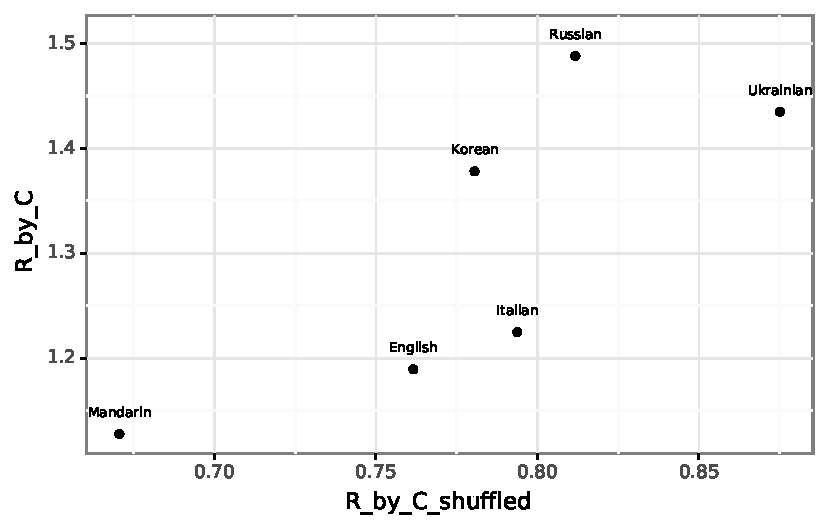
\includegraphics[width=\linewidth]{figures/ggplot_bible.pdf}
\caption{Complexity trade-offs for languages in the Parallel Bible Corpus $(R/C$  vs.~$R/C\textsubscript{shuffled})$}
\label{bible}
\end{figure}


\section{General discussion} \label{discussion}
\largerpage
Our analysis of word-order and word-structure complexity in heritage languages reveals some support for complexity trade-offs -- as operationalized by in\-for\-ma\-tion-the\-o\-ret\-ic compression-based metrics -- in the development of heritage languages. We saw that in Ukrainian, the language for which we have the most data, complexity trades off across the generations such that, as generational distance from the homeland increases, word-structure complexity decreases while word-order complexity increases. We found  support for a similar trade-off in Italian. The remaining languages in our analysis failed to yield reliable results that track heritage generations. 

\begin{sloppypar}
In an attempt to understand why Ukrainian may stand apart from the other languages in the clarity with which it demonstrates complexity trade-offs, we hypothesized that complexity trade-offs are precipitated by contact between two systems of markedly different morphological complexity. Ukrainian features high morphological complexity, while English's morphology is much simpler; when the two systems come into contact in a heritage speaker 
who winds up dominant in English, the result is morphological simplification in the Ukrainian grammar.
The results of our Bible analysis of the baseline grammars support this interpretation of the results, but we await a clearer picture from Korean and Russian~-- the two other languages where their morphological complexity relative to English leads us to expect trade-offs.\footnote{It would also be interesting to see what happens when the complexity asymmetry shifts in the opposite direction, such that the dominant language features much greater morphological complexity (as in, e.g., a Ukrainian-dominant heritage speaker of English). Unfortunately, such dyads are quite rare in the study of heritage languages \citep{ScontrasPutnam2020}.} 
While our dataset's small size is a limitation of our findings, we trust that, as data from multiple generations of heritage speakers become increasingly available, the picture of changing complexity in heritage grammars will become clearer still. Already our results suggest that, rather than being characterized only in terms of a general decrease in complexity relative to the baseline, in heritage languages, as in the languages analyzed by \citet{koplenig2017statistical}, complexity is changing in ways that lead to increases in some areas and decreases in others.\footnote{We also applied the entropy-based metrics from \citet{koplenig2017statistical} to our dataset, but we failed to find consistent relationships between word-order and word-structure complexity. We believe our dataset's small sample size could be one reason why we did not observe any clear trends from the entropy-based metrics, which rely on much larger samples to yield reliable results.}
\end{sloppypar}

This finding of complexity changes was anticipated by \citet{lalekoscontras2021}, who discuss the many ways that complexity may exist in heritage languages. We have focused here on morphological (word-structure) and syntactic (word-order) complexity,  finding evidence of a trading relationship between the two. Assuming researchers continue to find evidence of such trends across the generations of different heritage languages, it will be important to ask why morphology appears to be so susceptible to change, and why syntax should offer such a ready compensatory mechanism. However, these two notions -- morphological and syntactic complexity -- do not exhaust the many types of complexity that characterize a language and its usage. Grammars are complex systems with interacting components, and there are many other areas where complexity may be shifting (e.g., phonology, pragmatics, or several aspects of usage; see \citealp{lalekoscontras2021} for discussion). We leave it to future work to explore these other areas, in an effort to arrive at a full picture of complexity in heritage languages. 

\printbibliography[heading=subbibliography,notkeyword=this]

\end{document}
